\documentclass[a4paper]{article}
\usepackage[pdftex]{graphicx}
\usepackage[utf8]{inputenc}
\usepackage{enumerate}
\usepackage{icomma}
\usepackage{siunitx}
\sisetup{locale=DE}
\usepackage{amssymb}
\usepackage{tikz}
\usepackage{href-ul}
\hypersetup{
	colorlinks=true,
	linkcolor=blue,
	urlcolor=blue}
\usepackage{geometry}
\geometry{a4paper, top=15mm, left=15mm, right=15mm, bottom=15mm,
	headsep=10mm, footskip=12mm}

\begin{document}
	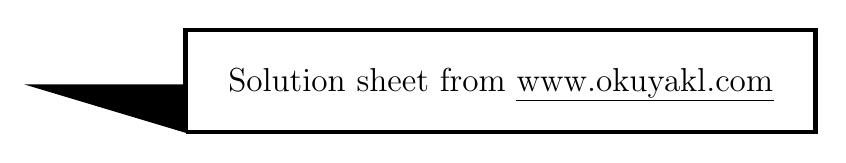
\begin{tikzpicture}(10,3)
		\draw[ultra thick](2,0) --(10,0) -- (10,1.3) --(2,1.3) -- (2,0);
		\draw[fill=black](2,0)-- (0,.6) -- (2,.6) -- (2,0);
		\node at (6,.6) {\large Solution sheet from \href{http://www.okuyakl.com}{www.okuyakl.com}};
	\end{tikzpicture}
	\vspace{0.5 cm}
	
	
	\noindent{\bf Task 1.}\\
	The blue area consists of two circle segments with the radius $a$ and the center angle $\mu = 90^\circ$ ({\it A circle segment is calculated with the area of a sector of a circle minus the area of the triangle}):
	$$ A_{blue}= 2 \cdot \left( {90^\circ \over 360^\circ} \cdot \pi \cdot a^2 - {1 \over 2}a^2 \right) =
	\left( {\pi \over 2} - 1 \right) \cdot a^2 $$
	\noindent{\bf Task 1. b)}\\
	The hatched area is also a circle segment with the center angle
	$\mu=90^\circ$, but with the radius
	$$r_s=\sqrt{a^2+a^2} = \sqrt{2} \cdot a$$
	The triangle area is $a^2$.
	$$A_{sch}= {90^\circ \over 360^\circ} \cdot \pi \cdot (\sqrt{2}a)^2 - a^2=
	{\pi \over 4} \cdot 2a^2- a^2 = \left({\pi \over 2} -1\right) \cdot a^2 = A_{blue}$$
	
	\noindent {\bf Task 2.}\\
	The area of the circle sector is:
	$$A_{KS}={\mu \over 360^\circ} \cdot \pi \cdot r^2 = {70^\circ \over 360^\circ}\cdot \pi \cdot ( \SI{4 }{\centi \meter})^2=\underline{\SI{9.77}{\centi \meter^2}}$$
	The area of triangle $ABM$ is:
	$$A_{\Delta}={1\over 2}r^2 \cdot \sin{\mu}={1\over 2}(\SI{4}{\centi\meter})^2 \cdot \ sin{70^\circ}=\underline{\SI{7,52}{\centi\meter^2}}$$
	The area of the circle sector is larger by this percentage relative to the area of the triangle:
	$$p={A_{KS} - A_{\Delta}\over A_{\Delta}}\cdot 100\% =\underline{30\%}$$
	
	\noindent
	\fbox{
		\begin{minipage}{0.47\textwidth}
			\noindent {\bf Task 3.}\\
			The circumference consists of two arcs plus the length of the radius.
			$$
			\renewcommand{\arraystretch}{2}
			\begin{array}{rcl}
				U &=& 2 \cdot b + r \\
				&=& 2 \cdot {60^\circ \over 180^\circ}\cdot \pi \cdot 1.5 +1.5 \\
				&=& 4.64~m
			\end{array}
			$$
			The area is made up of two circular sectors, from which an equilateral triangle must be subtracted.
			$$
			\renewcommand{\arraystretch}{2}
			\begin{array}{rcl}
				A &=& 2 \cdot A_{SEK} - A_\Delta \\
				&=& 2 \cdot {60^\circ \over 360^\circ} \cdot \pi 1.5^2 - {1\over 2} \cdot 1.5^2 \cdot \sin 60^\circ\\
				&=& 1.38~m^2
			\end{array}
			$$
		\end{minipage}}
	
	\noindent
	\fbox{
		\begin{minipage}{0.47\textwidth}
			\noindent {\bf Task 4.}\\
			The area is composed of an equilateral triangle of length $2r$ minus three sixths of a circle, i.e. a semicircle with radius $r$.
			$$
			\renewcommand{\arraystretch}{2}
			\begin{array}{rcl}
				A &=& A_\Delta - A_{HK}\\
				&=& {1 \over 2} \cdot (2r)^2 \cdot \sin(60^\circ)-{1\over 2} \pi r^2 \\
				&=& (\sqrt{3} - {1 \over 2}\pi)~r^2 \\
				&=& 0.16 \cdot r^2
			\end{array}
			$$
		\end{minipage}
	}
	\vspace{0.5 cm}
	
	
	\noindent {\bf Task 5.}\\
	We calculate: Area = Large sector of a circle minus semicircle plus small segment of a circle.\\
	Small circle segment = Small circle sector minus small equilateral triangle.
	$$
	\renewcommand{\arraystretch}{2}
	\begin{array}{rcl}
		A &=& A_{SEK}-A_{HK}+(A_{sek}-A_\Delta)= A_{SEK}-A_{HK}+A_{sek}-A_\Delta\\
		&=& {60^\circ \over 360^\circ}\cdot \pi (2r)^2-{1\over 2}\pi r^2 + {60^\circ \over 360^\circ}\ cdot \pi r^2- {1 \over 2} \cdot r^2 \cdot \sin(60^\circ)\\
		&=& ({2\over 3}\pi - {1\over 2}\pi +{1\over 6} \pi -{1 \over 4}\sqrt{3})~r^2= ({ 1\over 3} \pi - {1 \over 4}\sqrt{3})~r^2\\
		&=& 0.614~r^2
	\end{array}
	$$
	
\noindent{\bf Task 6. a)}\\
Two equilateral triangles with side length $a$ can be inscribed in the figure. The outer lens shape consists of two circle segments with radius $a$ and center angle $\mu=120^\circ$ .
Such a circle segment has the area:
$$A_1={\mu \over 360^\circ}\cdot \pi a^2 - {1\over 2} a^2 \cdot \sin{\mu}={\pi \over 3} a^2 -{\sqrt{3}\over 4} a^2$$
The iris is a circle with radius $a/2$. Your area is:
$$A_2=\pi \cdot \left({a \over 2}\right)^2 = {\pi \over 4} a^2$$
The pupil is composed of two circle segments with radius $a$ and center angle $\mu=60^\circ$:
$$A_3={\mu \over 360^\circ}\cdot \pi a^2 - {1\over 2} a^2 \cdot \sin{\mu}={\pi \over 6} a^2 -{\sqrt{3}\over 4} a^2$$
The entire blue area consists of:
$$
\renewcommand{\arraystretch}{2}
\begin{array}{rcl}
	A_{tot} &=& 2\cdot A_1 - A_2 + 2 \cdot A_3\\
	A_{tot} &=& 2(\cdot {\pi \over 3} a^2-{\sqrt{3}\over 4}a^2) - {\pi \over 4} a^2 + 2( {\pi \over 6} a^2-{\sqrt{3}\over 4} a^2 )\\
	A_{tot} &=& a^2 \cdot ( {2 \pi \over 3} -{\sqrt{3}\over 2}- {\pi \over 4}+{\pi \over 3}-{ \sqrt{3}\over 2})\\
	A_{tot} &=& a^2 \cdot ({3 \pi \over 4}-\sqrt{3})\quad (*)
\end{array}
$$

\noindent{\bf Task 6. b)}\\
We substitute $a=\SI{8}{\centi\meter}$ into $(*)$ and get:
$$A_{ges}= (\SI{8}{\centi\meter})^2 \cdot ({3 \pi \over 4}-\sqrt{3})= \SI{64}{\centi\ meter^2}\cdot 0.624 = \SI{39.9}{\centi\meter^2}$$

\begin{center}
	\includegraphics[width=7 cm]{../../viecher/eendcomic.pdf}
	
	Here you can go back to the \href{https://www.okuyakl.de/math/m10kreibL027/ae027.pdf}{Task sheet}
\end{center}

\end{document}